\documentclass[11pt,a4paper]{article}

\usepackage[polish]{babel}
\usepackage[utf8]{inputenc}
\usepackage{polski}
\usepackage[T1]{fontenc}
\usepackage{indentfirst}
\usepackage{wrapfig}    % for wrapping figures, tables

\frenchspacing

%\usepackage{amsmath}
\usepackage{physics}
%\usepackage{bm}
\usepackage{gensymb}
%\usepackage{hepnames}
\usepackage{epsfig}
\usepackage{graphics}
\usepackage[shortlabels]{enumitem}
%\usepackage{xspace}
%\xspaceaddexceptions{[]\{\}}

%
%
%fixpagesize
\pagestyle{empty}
\addtolength{\textwidth}{6cm}
\addtolength{\textheight}{4cm}
\addtolength{\evensidemargin}{-3cm}
\addtolength{\oddsidemargin}{-3cm}
\addtolength{\topmargin}{-2cm}
\parindent=0cm

%
%
%small distance in list/item/enum for enumitem package
\setlist[itemize,enumerate]{topsep=0em}
\setlist{noitemsep}


% definition of inexact differential symbol:
\newcommand{\dbar} {\ensuremath{\,\mathchar'26\mkern-12mu d}}

%print zadanie #
\newcounter{zadanie}\newcommand{\zadanie}[1][]{\addtocounter{zadanie}{1} ~\\  {\bf \emph{Zadanie \arabic{zadanie} #1 }} \\}
\newcounter{zaddom}\newcommand{\zaddom}[1][]{\addtocounter{zaddom}{1} ~\\  {\bf \emph{Zadanie domowe \arabic{zaddom} #1 }} \\}
%\renewcommand{\zadanie}[1][]{\pagebreak  ~\\  {\bf \emph{Zadanie }} \\} \addtolength{\topmargin}{-2cm}


%
%%%%%%%%%%%%%%%%%%%%%%%%%%%%%%%%%%%%%%%%%%%%%%%%%%%%%%
% Changes figure placing algorithm
\renewcommand{\topfraction}{1}       % maximal fraction of a page allowed for figures
\renewcommand{\textfraction}{0.15}   % minimal number of text for figure-text shared pages
\renewcommand{\floatpagefraction}{0.95} % if two above does not help, this could do the job
                                        % must be: floatpagefraction < topfraction !!!!
%
\renewcommand{\textfraction}{0} % minimum fraction of page, which must be
                                % devoted to text
\renewcommand{\topfraction}{1}  % maximum fraction at top, which can be
                                % occupied whit floats
\setcounter{totalnumber}{400}   % increase the number of floats for one page
\setcounter{topnumber}{200}     % at all/top/bottom.
\setcounter{bottomnumber}{200}  %


\begin{document}           % End of preamble and beginning of text.
\begin{centering}
\bf{\Large{Termodynamika z elementami fizyki statystycznej}}\\
Tydzień 12 (25 maja 2023)\\[5mm]
Rozkład Boltzmanna, entropia \\
\end{centering} 
\vspace{5mm}

\begin{wrapfigure}[3]{r}{0.2\linewidth}\vspace{-5mm}
\resizebox{\linewidth}{!}{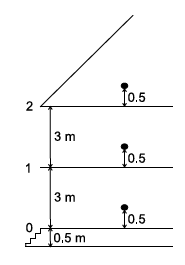
\includegraphics{szewc.png}}
\end{wrapfigure}
\zadanie
Szewc ma na rynku wąski domek o 3 kondygnacjach. W ciągu doby średnio:
\begin{itemize}
\item 4 h 35 min. spędza w kuchni na 2 piętrze,
\item 7 h 25 min. śpi w sypialni na 1 piętrze,
\item 12 h pracuje w warsztacie na parterze.
\end{itemize}
(a) Jakie jest prawdopodobieństwo znalezienia szewca na poziomie 0, 1 oraz 2?\\
(b) Jaka jest średnia wysokość środka masy szewca w ciągu doby (patrz rysunek)?\\
(c) Jaka jest średnia energia potencjalna szewca ($m=50$ kg)?\\
(d) Czy opisany układ mógłby być rozkładem termicznym? \\

\zadanie
Pewna cząsteczka ma, poza stanem podstawowym o zerowej energii, dwa stany wzbudzone o energiach $\varepsilon$ i $2\,\varepsilon$.
Obserwując 1 mol takich (rozróżnialnych) cząsteczek stwierdzono, że w wymienionych stanach przebywa odpowiednio 4/7, 2/7 i 1/7 cząsteczek.
\begin{enumerate}[a)]
\item Znajdź entropię układu licząc mikrostany. 
\item Znajdź entropię korzystając ze wzoru Gibbsa.
\end{enumerate}
Stała Boltzmanna wynosi $k = 1.38\cdot 10^{-23}\,$J/K, 
liczba Avogadra $N_A=6.02\cdot 10^{23}$\, mol$^{-1}$. \\
%$R=8.31$\,J/mol/K. 
Jaki jest zakres stosowalności wzorów z pkt. a) i b)?

\zadanie
Pewna cząsteczka ma, poza stanem podstawowym o zerowej energii, dwa stany wzbudzone o energiach $\varepsilon$ i $2\,\varepsilon$.
Obserwując zespół wielu takich cząsteczek pozostających w równowadze z 
termostatem stwierdzono, że średnio 4/7 z nich jest w stanie podstawowym.
\begin{enumerate}[a)]
\item Jaka jest temperatura układu? 
      Jaki ułamek cząsteczek jest w stanie najwyższego wzbudzenia?
\item W powyższym układzie znalazła się jedna cząsteczka innego typu, 
      mająca dwa różne stany wzbudzone, ale oba o tej samej energii $2\,\varepsilon$. 
      Jakie jest prawdopodobieństwo znalezienia jej w stanie podstawowym?
\end{enumerate}


\zadanie
{\em Dwupoziomowy (kwantowy) model paramagnetyzmu}\\
W jednorodnym zewnętrznym polu magnetycznym o indukcji $\vec{B}$
znajduje się atom o spinie $\frac{1}{2}$ i momencie magnetycznym $\vec{\mu}_0$.
Moment magnetyczny atomu może być ustawiony albo równolegle albo antyrównolegle do
zewnętrznego pola magnetycznego, a energia oddziaływania z tym polem wynosi
$\displaystyle E = - \vec{\mu}_0 \cdot \vec{B}$.
Układ znajduje się w równowadze z termostatem o temperaturze $T$.
\begin{enumerate}[a)]
\item Obliczyć średni moment magnetyczny atomu,
\item Przedyskutować wynik w granicy $\mu_0 B \gg k T$ (tj. silne pole, niska temperatura) oraz $\mu_0 B \ll k T$ (tj. słabe pole, wysoka temperatura),
\item Pamiętając, że: podatnością magnetyczną $\chi$ nazywa się współczynnik proporcjonalności między namagnesowaniem materiału $\vec{M}$ a polem $\vec{B}$,
zaś namagnesowanie $\vec{M}$ jest momentem magnetycznym na jednostkę 
objętości materiału, wykazać, że w granicy słabych pól magnetycznych dla naszego modelowego paramagnetyka spełnione jest prawo Curie:
$\displaystyle \chi = \frac{C}{T}$,
gdzie $C$ jest pewną stałą, nazywaną stałą Curie.
\end{enumerate}

\pagebreak
\zadanie
Udowodnij, że dla cząstki będącej w równowadze z termostatem o temperaturze $T$ i 
podlegającej rozkładowi Boltzmanna spełnione są tożsamości:
\[ \langle E\rangle = - \frac{1}{Z} \cdot \frac{\partial Z}{\partial \beta}, ~~~~
\langle E^2\rangle = \frac{1}{Z} \cdot \frac{\partial^2 Z}{\partial \beta^2}, \]
gdzie: $E$ - energia cząstki, $Z$ - suma statystyczna, $\beta = \frac{1}{k T}$.
Rozważ przypadki dyskretnych i ciągłych stanów energetycznych.

\zadanie
Energie stanów rotacyjnych cząsteczek dwuatomowych dane są wzorem: $E_j = j(j+1)\varepsilon$,
gdzie $j=0,1,2,...$, a $\varepsilon$ jest stałą. 
Dla każdej warości $j$  występuje $2j+1$ różnych stanów o tej samej energii $E_j$. 
Oblicz średnią energię takiej cząsteczki w warunkach równowagi termodynamicznej 
z termostatem o temperaturze $T$ przy założeniu, że $kT \gg \varepsilon$, gdzie $k$ - stała Boltzmanna.


%
% domowe 
%

\zaddom
Cząstki pewnego układu mogą zajmować tylko trzy następujące stany energetyczne:\linebreak
jeden stan podstawowy o energii 0, dwa stany o energii $\varepsilon$
 i trzy stany o energii $2\varepsilon$. Stwierdzono, że
w warunkach równowagi termodynamicznej średnia energia jednej cząstki
jest równa $2\varepsilon/3$.
Jaka jest temperatura układu?
Jakie jest prawdopodobieństwo znalezienia cząstki o energii $\varepsilon$?
\\
\textit{Odpowiedź:} $T=\varepsilon/(k_B  \ln 3), \, P(\epsilon)=1/3$

\zaddom
W chmurach gazu międzygwiezdnego znajdują się czasem molekuły cyjanu (CN). W cząsteczce
tej, przy energii $4.7 \cdot 10^{-4}$\,eV powyżej stanu podstawowego, znajdują się trzy najniżej leżące
rotacyjne stany wzbudzone. Astronomiczne pomiary spektroskopowe wykazały, że w pewnej
chmurze średnio na każde 10 cząstek CN w stanie podstawowym, 3 inne cząstki znajdują się w
jednym z tych trzech stanów wzbudzonych. Oblicz temperaturę tej chmury.
\\
\textit{Odpowiedź:}$T\approx 2.3 K$

\zaddom
Cząstki pewnego układu mogą występować tylko w dwóch stanach:
w stanie podstawowym o energii 0 i w stanie wzbudzonym o energii $\varepsilon$.
W stanie podstawowym cząstka ma wartość składowej z momentu pędu $J_z=-\frac{1}{2}$, a w stanie wzbudzonym $J_z=\frac{1}{2}$.
Stwierdzono, że w stanie równowagi średnia wartość energii jednej cząstki wynosi $\langle E\rangle = \varepsilon/4$. Jaka jest temperatura układu?
Oblicz średnią wartość składowej $J_z$ momentu pędu jednej cząstki.
\\
\textit{Odpowiedź:} $T=\varepsilon/(k_B \ln 3), \, \langle J_z \rangle = -\frac{1}{4}$

%\zaddom
%Stała dielektryczna $\varepsilon$ wyraża się wzorem:
%$\displaystyle \varepsilon = 1 + \frac{N \langle p_{ez}\rangle}{\varepsilon_0 E_{el}}$,
%gdzie $N$ jest liczbą cząsteczek na jednostkę objętości,
%$E_{el}$ -- natężeniem pola elektrycznego,
%zaś $\langle p_{ez}\rangle$ -- średnim rzutem elektrycznego momentu dipolowego cząsteczek ośrodka na kierunek pola elektrycznego $\vec{E}_{el}$.
%Doświadczalnie stwierdzono, że stała dielektryczna $\varepsilon$ gazów,
%których cząsteczki mają niezerowy trwały moment dipolowy $\vec{p}_{e}$
%jest liniową funkcją odwrotności temperatury.
%Oznacza to, że $\langle p_{ez} \rangle$ także powinnien być liniową funkcją
%odwrotności temperatury.
%Wiedząc, że energia potencjalna dipola elektrycznego w jednorodnym polu
%elektrycznym $\vec{E}_{el}$
%dana jest wzorem: $E_p = - \vec{p}_{e} \cdot \vec{E}_{el}$
%obliczyć średnią wartość rzutu elektrycznego momentu dipolowego
%$\langle p_{ez}\rangle$ w polu elektrycznym, w równowadze z
%termostatem o temperaturze $T$.
%Wykazać, że w granicy $E_{el}/T \rightarrow 0$ (tj. słabe pole, wysoka
%temperatura) wynik ten jest proporcjonalny do $1/T$.
%

\zaddom
Na ćwiczeniach rozważaliśmy dwupoziomowy, kwantowy model paramagnetyzmu, w którym
zakładaliśmy, że możliwe są tylko dwie różne wartości rzutu momentu magnetycznego
$p_m = \mu_0$
atomu o spinie $\frac{1}{2}$ na oś pola magnetycznego (tj. $\pm \mu_0$).
Jaki wynik na średni rzut momentu magnetycznego $<p_{mz} >$
otrzymalibyśmy dla „klasycznej igły magnetycznej”, dla której
moment magnetyczny może przyjmować dowolny kierunek w przestrzeni?\\
\textit{Wskazówka: Jest to tzw. model paramagnetyzmu Langevin. Prawdopodobieństwo znalezienia momentu magnetycznego pod kątem $\theta$ do kierunku pola magnetycznego} $\sim e^{\mu_0B \beta} \sin \theta d \theta$
\\
\textit{Odpowiedź:} $\langle p_{mz} \rangle=\mu_0 [\coth (\mu_0 B \beta)-\frac{1}{\mu_0B \beta} ]$

\zaddom
Suma statystyczna pewnego układu spełnia zależność $\ln{Z} = a T^4 V$,
gdzie $a$ jest pewną stałą, $T$ oznacza temperaturę, zaś $V$ objętość.
Wyznacz pochodną średniej energii po temperaturze przy stałej objętości
tego układu (tzn. pojemność cieplną).
\\
\textit{Odpowiedź:} $\left(\frac{\partial U}{\partial T}\right)_V=20k_baT^4V$


% An example of figure placement:
%\begin{wrapfigure}[13]{r}{0.4\linewidth}\vspace{3mm}
%\resizebox{\linewidth}{!}{\includegraphics{NAZWA.png}}
%\end{wrapfigure}
%\zaddom

\end{document}
